% !TeX program = lualatex
\documentclass[UTF8,zihao=-4,fontset=fandol]{ctexart}
\usepackage[a4paper,top=2.1cm,bottom=2.3cm,left=2.3cm,right=2.3cm]{geometry}
\usepackage{amsmath,amssymb,bm,booktabs,array,graphicx,caption,float,enumitem,longtable}
\usepackage{fancyhdr,microtype,setspace,url}
\graphicspath{{output/pdf/wang2011_zh_figures/}{wang2011_zh_figures/}}
\setstretch{1.20}\setlength{\parindent}{2em}\setlength{\parskip}{0.16em}\setlength{\headheight}{14pt}
\captionsetup{font=small,labelsep=quad}
\pagestyle{fancy}\fancyhf{}
\fancyhead[L]{\small 铝电解槽电解质中流动相关现象的模拟}
\fancyhead[R]{\small Wang 等（2011）}\fancyfoot[C]{\thepage}
\ctexset{section={format=\large\bfseries,name={},number=\Roman{section}.,aftername=\quad},subsection={format=\normalsize\bfseries,name={},number=\Alph{subsection}.,aftername=\quad}}
\newcommand{\vect}[1]{\bm{#1}}
\title{\bfseries 铝电解槽电解质中流动相关现象的模拟\\
\large Simulation of the Fluid Flow-Related Phenomena\\in the Electrolyte of an Aluminum Electrolysis Cell}
\author{Yufeng Wang，Lifeng Zhang\textsuperscript{*}，Xiangjun Zuo\\[0.5em]
\small 密苏里科技大学材料科学与工程系\\
\small\textsuperscript{*}\texttt{zhanglife@mst.edu}}
\date{\small \emph{Metallurgical and Materials Transactions B}, 42B (2011), 1051--1064\\
\url{https://doi.org/10.1007/s11663-011-9531-4}}
\begin{document}\maketitle\thispagestyle{empty}
\begin{center}\small\itshape 中文翻译稿；章节、公式、图和表的编号与原文逐一对应。\end{center}
\begin{abstract}
本文采用全尺寸水模型和数学模拟研究铝电解槽水模型中的流动相关现象。建立了瞬态多相流模型，用以表征电解质中的复杂非稳态流动，并通过水模型中的墨水扩散和激光多普勒测速（LDV）验证模型准确性。数值计算预测了大气泡的形态、运动与释放频率、液体流型以及电解质-金属界面。研究还讨论了阳极边缘圆角、底面倾角、开槽和电流密度等设计及运行因素。结果表明，圆角、开槽和倾斜底面联合使用有利于气泡逸出，并能提高电解质-金属界面的稳定性。
\end{abstract}
\noindent\textbf{关键词：}铝电解；水模型；VOF；气泡释放；阳极设计；电解质-金属界面

\section{引言}
Hall-H\'eroult 法是原铝生产的主要工业过程。氧化铝溶于熔融冰晶石电解质，直流电通过整个电解槽；液态铝沉积在槽底，而 CO 和 CO$_2$ 在阳极底面生成。阳极下的非导电气体增加阳极与阴极之间的总电阻。气泡可覆盖阳极底面积的 50\%--90\%，造成约 0.15--0.35 V 的平均电压降；若形成连续气膜，则可能引发阳极效应。稳定高效运行依赖于阳极气泡及时移除以及电解质-金属界面振荡得到控制。

关键因素包括气泡的成核、生长、运动、相互作用、聚并和脱离；阳极材料、尺寸、形状、开槽及边缘曲率；电解质化学组成与氧化铝溶解；以及电压、电流密度、阳极-阴极距离（ACD）和阳极倾角等运行参数。由于真实槽内环境高温、腐蚀性强，工业测量只能得到电流变化、界面波动和温度等有限信息，无法直接测量阳极下气膜。

水模型透明、安全、成本低，可借助摄影、LDV 或粒子图像测速观察气泡和液流，已广泛用于研究阳极下气泡。数值模型则可预测复杂流型。电解槽传质与传热受 MHD、气泡驱动力和温度梯度共同控制；在电解质局部，气泡驱动力通常占主导。二维瞬态模型无法反映阳极槽缝对不同位置气泡释放的影响，因此本文建立三维瞬态多相模型，并用水模型验证，系统考察阳极圆角、倾角和槽缝对气泡运动、释放频率、流型与界面稳定性的影响。

\begin{figure}[H]\centering
\includegraphics[width=.62\textwidth]{fig01.png}
\caption{铝电解槽内的主要现象。}\end{figure}

\section{研究方法}
\subsection{水模型}
水与冰晶石运动黏度接近，因此空气-水体系可近似模拟冰晶石-CO/CO$_2$ 体系。模型代表现代电解槽中的一个阳极单元：有机玻璃槽内悬挂两个长 1500 mm、宽 170 mm、高 430 mm 的箱体，形成带底部槽缝的阳极。ACD、阳极倾角和槽缝尺寸均可调。本文关注大气泡片的脱离，忽略小气泡成核与早期运动，通过 16 根直径 4 mm 的塑料管注气。

按法拉第定律，每通过 4 mol 电子生成 1 mol CO$_2$，单位阳极面积的产气率为
\begin{equation}q=\frac{iRT}{4FP}.\tag{1}\end{equation}
其中 $i$ 为阳极电流密度，$R=8.314~\mathrm{J/(mol\,K)}$，$T=1223~\mathrm{K}$，$F=96486~\mathrm{A\,s/mol}$，$P=101325~\mathrm{Pa}$，从而 $q=2.6\times10^{-7}i$。模型气量取 16--157 L/min，对应电流密度 0.2--2.0 A/cm$^2$。

\begin{figure}[H]\centering
\includegraphics[width=.86\textwidth]{fig02.png}
\caption{水模型：（a）俯视示意图；（b）实物图；（c）单位面积产气率与电流密度的关系。}\end{figure}

\begin{table}[H]\centering\caption{水与冰晶石的物性。}
\begin{tabular}{lcc}\toprule 参数&冰晶石&水\\\midrule 温度/K&1223&298\\密度/$\mathrm{kg\,m^{-3}}$&2100&1000\\运动黏度/$\mathrm{m^2s^{-1}}$&$1.4\times10^{-6}$&$1.0\times10^{-6}$\\表面张力/$\mathrm{N\,m^{-1}}$&0.5&0.073\\\bottomrule\end{tabular}\end{table}

使用录像测量气泡几何形态、轨迹和覆盖面积；用蓝色墨水示踪流型；采用二维 LDV 逐点测量瞬时速度。每个测点对约 1000 个颗粒、5--8 min 的数据取平均。侧部通道测量超过 300 点，阳极下方超过 100 点。单位质量湍动能由水平和竖直速度脉动计算：
\begin{equation}k=\frac12\left(\overline{u'^2}+\overline{v'^2}\right).\tag{2}\end{equation}

\begin{figure}[H]\centering
\includegraphics[width=.68\textwidth]{fig03.png}
\caption{LDV 测量区域。}\end{figure}

\subsection{数学模型}
采用标准 $k$-$\varepsilon$ 两方程模型描述瞬态多相湍流。连续方程为
\begin{equation}\frac{\partial\rho}{\partial t}+\frac{\partial(\rho u_i)}{\partial x_i}=0.\tag{3}\end{equation}
Navier-Stokes 方程为
\begin{equation}
\rho\frac{\partial u_i}{\partial t}+\rho\frac{\partial(u_i u_j)}{\partial x_j}
=-\frac{\partial p}{\partial x_i}+\frac{\partial}{\partial x_j}\left(\mu_{\rm eff}\frac{\partial u_i}{\partial x_j}\right)
+\frac{\partial}{\partial x_j}\left(\mu_{\rm eff}\frac{\partial u_j}{\partial x_i}\right)+\rho g_i+F_i.\tag{4}
\end{equation}
$F_i$ 可用于加入电磁力等动量源项。湍动能及其耗散率方程为
\begin{align}
\frac{\partial(\rho k)}{\partial t}+\frac{\partial}{\partial x_i}\left(\rho u_i k-\frac{\mu_{\rm eff}}{\sigma_k}\frac{\partial k}{\partial x_i}\right)
&=\mu_t\frac{\partial u_j}{\partial x_i}\left(\frac{\partial u_i}{\partial x_j}+\frac{\partial u_j}{\partial x_i}\right)-\rho\varepsilon,\tag{5}\\
\frac{\partial(\rho\varepsilon)}{\partial t}+\frac{\partial}{\partial x_i}\left(\rho u_i\varepsilon-\frac{\mu_{\rm eff}}{\sigma_\varepsilon}\frac{\partial\varepsilon}{\partial x_i}\right)
&=C_1\mu_t\frac{\varepsilon}{k}\frac{\partial u_j}{\partial x_i}\left(\frac{\partial u_i}{\partial x_j}+\frac{\partial u_j}{\partial x_i}\right)-C_2\rho\frac{\varepsilon^2}{k}.\tag{6}
\end{align}
湍流黏度为
\begin{equation}\mu_t=\rho C_\mu\frac{k^2}{\varepsilon}.\tag{7}\end{equation}
VOF 方法通过体积分数 $f_i$ 捕捉自由界面：
\begin{equation}\frac{\partial f_i}{\partial t}+\frac{\partial(f_i u_i)}{\partial x_i}=0.\tag{8}\end{equation}
当单元内无目标流体时 $f=0$，完全充满时 $f=1$，界面单元满足 $0<f<1$。二维和三维结构网格分别约 48.5 万和 66 万单元，采用 FLUENT 非稳态求解器与 VOF 模型。压力-速度耦合用 PISO，动量和湍流量采用二阶迎风格式，体积分数采用几何重构。

\begin{figure}[H]\centering
\includegraphics[width=.94\textwidth]{fig04.png}
\caption{二维计算几何与边界：（a）90$^\circ$ 阳极边缘；（b）圆弧阳极边缘。}\end{figure}
\begin{figure}[H]\centering
\includegraphics[width=.68\textwidth]{fig05.png}
\caption{三维计算域及边界。}\end{figure}

\section{模型验证}
墨水在水模型侧部通道形成明显回流：靠近阳极侧向上、靠近槽壁向下。三维模型所得流型与墨水示踪一致（图 6），LDV 测得的速度矢量与计算结果也吻合（图 7）。水模型和数值模拟均显示阳极下形成展平的大气泡片，三维模型正确再现了气泡纵向尺度、运动方向和槽缝释放路径。二维模型能够预测侧视形态，但三维模型对气泡长度、覆盖率及槽缝作用的描述更可靠。

\begin{figure}[H]\centering
\includegraphics[width=.94\textwidth]{fig06.png}
\caption{侧部通道回流：（a）水模型墨水示踪；（b）三维模拟流型。}\end{figure}
\begin{figure}[H]\centering
\includegraphics[width=.94\textwidth]{fig07.png}
\caption{速度矢量分布：（a）LDV 测量；（b）三维模拟。}\end{figure}
\begin{figure}[H]\centering
\includegraphics[width=.94\textwidth]{fig08.png}
\caption{气泡形态：（a）水模型侧视；（b）水模型底视；（c）三维模拟；（d）气泡纵向尺寸。}\end{figure}
\begin{figure}[H]\centering
\includegraphics[width=.94\textwidth]{fig09.png}
\caption{阳极倾角 1.1$^\circ$ 时不同时间的墨水扩散。}\end{figure}

\section{气体流量的影响}
提高气体流量使阳极下气泡更快生长、聚并和释放，并强化侧部通道回流与自由表面乳化。低气量时气泡片较薄、释放间隔较长；高气量时大气泡片更频繁越过阳极边缘，自由表面扰动明显增强。水模型和数值结果具有一致趋势。
\begin{figure}[H]\centering
\includegraphics[width=.94\textwidth]{fig10.png}
\caption{气体入口速度对气泡运动与自由表面乳化的影响：（a）0.5 m/s；（b）1.0 m/s。}\end{figure}

\section{阳极边缘形状的影响}
直角阳极边缘会阻碍气泡绕过边缘，使大气泡在底面滞留并积聚；圆弧边缘减小局部阻力，使气泡更连续地沿边缘上升，降低阳极下气体覆盖率。圆角还能减弱气泡突然脱离造成的液体脉动，因此更有利于界面稳定。
\begin{figure}[H]\centering
\includegraphics[width=.74\textwidth]{fig11.png}
\caption{阳极边缘形状对气泡运动的影响：（a）直角；（b）圆角。}\end{figure}
\begin{figure}[H]\centering
\includegraphics[width=.58\textwidth]{fig12.png}
\caption{阳极槽缝构型。}\end{figure}

\section{阳极倾角与槽缝的影响}
水平阳极下气泡运动缓慢，聚并为大气泡片后主要由槽缝逸出；阳极底面倾斜后，浮力沿底面的分量推动气泡向高侧运动。1.1$^\circ$ 倾角使回流更强、气体覆盖率降低，且气泡可同时从槽缝和阳极边缘逸出。槽缝为气泡提供替代排放路径，与倾角联合使用最为有效。

\begin{figure}[H]\centering
\includegraphics[width=.86\textwidth]{fig13.png}
\caption{不同时间的墨水扩散：（a）1 s；（b）5 s；（c）10 s。}\end{figure}
\begin{figure}[H]\centering
\includegraphics[width=.96\textwidth]{fig14.png}
\caption{不同阳极倾角下的测量速度与湍动能。}\end{figure}
\begin{figure}[H]\centering
\includegraphics[width=.96\textwidth]{fig15.png}
\caption{侧部通道阳极中心平面上的三维速度与流线。}\end{figure}
\begin{figure}[H]\centering
\includegraphics[width=.96\textwidth]{fig16.png}
\caption{阳极底面气泡释放：（a,b）倾角 0$^\circ$；（c,d）倾角 1.1$^\circ$；实验与模拟对照。}\end{figure}
\begin{figure}[H]\centering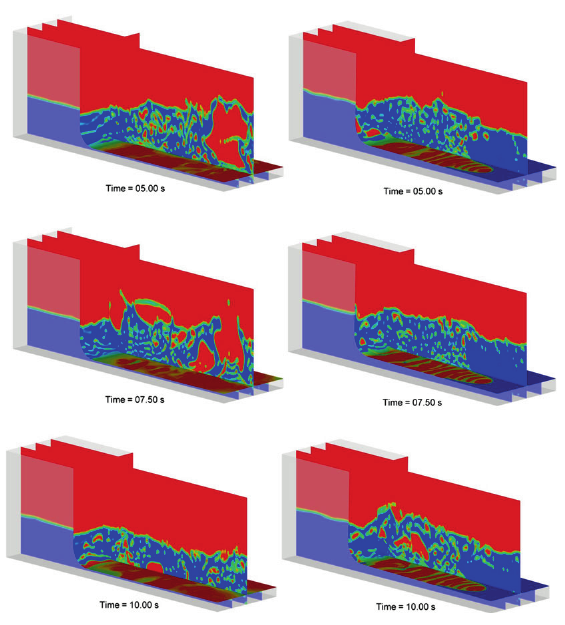
\includegraphics[width=.72\textwidth]{fig17.png}
\caption{阳极底面气泡释放与覆盖状态。}\end{figure}

\section{气泡释放频率}
工业电解槽通常根据电压或电流波动统计释放频率，正常电流密度下约为 0.5--3 Hz。瞬态模型中，局部速度随时间的变化可作为气泡释放指标：大气泡释放导致较大速度脉动，小气泡影响较弱。水平阳极需 4--8 s 才进入准稳定释放，频率约 1 Hz；1.1$^\circ$ 倾斜阳极约 3 s 即达到准稳定，频率约 1.5 Hz。较高频率对应较小的阳极下气泡尺寸。
\begin{figure}[H]\centering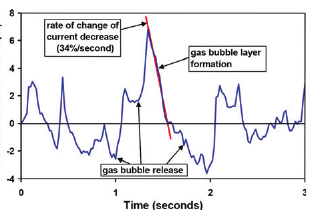
\includegraphics[width=.66\textwidth]{fig18.png}
\caption{工业无槽阳极电流随时间的典型变化及气泡释放事件（50 Hz 采样）。}\end{figure}
\begin{figure}[H]\centering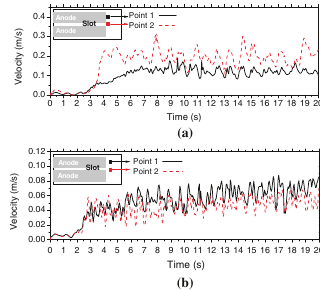
\includegraphics[width=.82\textwidth]{fig19.png}
\caption{气泡释放频率：（a）阳极倾角 0$^\circ$；（b）1.1$^\circ$。}\end{figure}

\section{电解质-铝液界面压力}
气泡驱动流和 MHD 流都会使电解质-金属界面振荡。忽略界面运动的动态效应时，可由局部压力相对于平均压力的差计算界面相对高度：
\begin{equation}
\Delta h=\frac{p_{\rm local}-p_{\rm mean}}{g(\rho_{\rm metal}-\rho_{\rm electrolyte})}.\tag{9}
\end{equation}
计算表明，水平阳极下气泡聚集造成更大的压力不均匀和界面起伏；倾斜阳极使气泡更快释放，界面更平稳。
\begin{figure}[H]\centering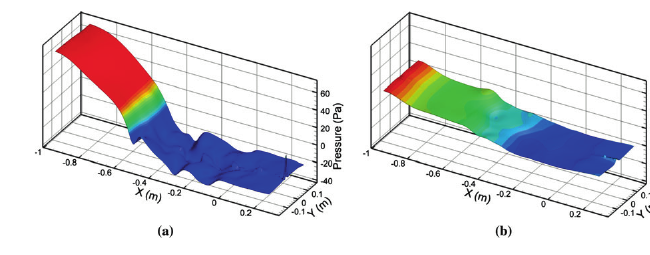
\includegraphics[width=.94\textwidth]{fig20.png}
\caption{注气 10 s 后由压力差预测的金属-电解质界面：（a）倾角 0$^\circ$；（b）1.1$^\circ$。}\end{figure}

\section{结论}
\begin{enumerate}[label=\arabic*.]
\item 三维瞬态多相模型能够预测水模型中气泡运动、气泡释放、液体循环及界面响应，并得到墨水示踪和 LDV 测量验证。
\item 阳极下气泡呈扁平片状，三维模型比二维模型更适合预测其长度、覆盖率和槽缝释放路径。
\item 侧部通道形成靠阳极上升、靠外壁下降的回流；增加阳极倾角会强化该循环。
\item 圆弧阳极边缘促进气泡平顺越过边缘，降低滞留和气体覆盖；槽缝为气泡提供重要排放通道。
\item 水平阳极气泡释放频率约 1 Hz，1.1$^\circ$ 倾斜阳极约 1.5 Hz；倾角提高可缩短达到准周期状态的时间。
\item 气泡驱动压力会引起电解质-金属界面变形；倾斜阳极的界面波动较小。
\item 圆角、槽缝和倾斜底面组合是兼顾气泡排放和界面稳定性的有效阳极设计。
\end{enumerate}

\section*{致谢}
作者感谢美国国家科学基金会、密苏里科技大学材料研究中心以及相关工业合作方的支持。

\section*{参考文献}
\small 原文共列出 47 篇参考文献，涵盖 Aaberg、Fortin、Shekhar、Evans、Kiss、Cooksey、Feng、Thomas、Launder 和 Spalding 等关于铝电解气泡、水模型、VOF、湍流及界面动力学的研究。为保持引文对应关系，正文中的文献序号均与英文原文一致；完整书目信息见原文参考文献表。

\vfill\begin{center}\footnotesize 翻译依据：Wang, Zhang and Zuo, \emph{Metallurgical and Materials Transactions B}, 42B (2011), 1051--1064。\end{center}
\end{document}
